% A-14 architecture overview and request loop; the report includes the committed architecture.pdf.
% Needs the tgheros and sourcecodepro packages. Build outside the repository: pdflatex architecture.tex
\documentclass[tikz,border=6pt]{standalone}
\usepackage[T1]{fontenc}
\usepackage{tgheros}
\usepackage[scale=0.85]{sourcecodepro}
\renewcommand{\familydefault}{\sfdefault}
\usetikzlibrary{arrows.meta,fit,backgrounds,calc}

\definecolor{ink}{HTML}{1F2A44}
\definecolor{line}{HTML}{5B6478}
\definecolor{muted}{HTML}{6B7280}
\definecolor{band}{HTML}{F3F4F6}
\definecolor{wire}{HTML}{C9CED6}
\definecolor{accent}{HTML}{B4561F}
\definecolor{accentbg}{HTML}{FBF0E8}
\definecolor{focus}{HTML}{EAF0F7}

\tikzset{
  every node/.style={font=\footnotesize, text=ink},
  box/.style={draw=ink, line width=0.7pt, rounded corners=3pt, fill=white, align=center,
    text width=2.2cm, minimum height=1.15cm, inner sep=3pt},
  guard/.style={box, draw=accent, fill=accentbg, text width=1.9cm},
  chip/.style={draw=line, line width=0.5pt, rounded corners=2pt, fill=white, align=center,
    font=\scriptsize, inner sep=2.5pt},
  area/.style={draw=line!55, line width=0.6pt, rounded corners=6pt, fill=band},
  atitle/.style={anchor=north west, inner sep=6pt},
  flow/.style={-{Latex[length=2.8mm, width=2.2mm]}, draw=ink, line width=1.5pt},
  call/.style={{Latex[length=2.2mm]}-{Latex[length=2.2mm]}, draw=line, line width=1pt},
  lbl/.style={font=\scriptsize, inner sep=2pt},
  tag/.style={draw=ink, rounded corners=1.5pt, font=\sffamily\bfseries\footnotesize, text=ink, inner sep=1.6pt, fill=white},
}
\newcommand{\bx}[2]{\textbf{#1}\\[1pt]{\scriptsize\color{muted}#2}}
\newcommand{\tagged}[2]{\node[tag] at (#1.north west) {#2};}

\begin{document}
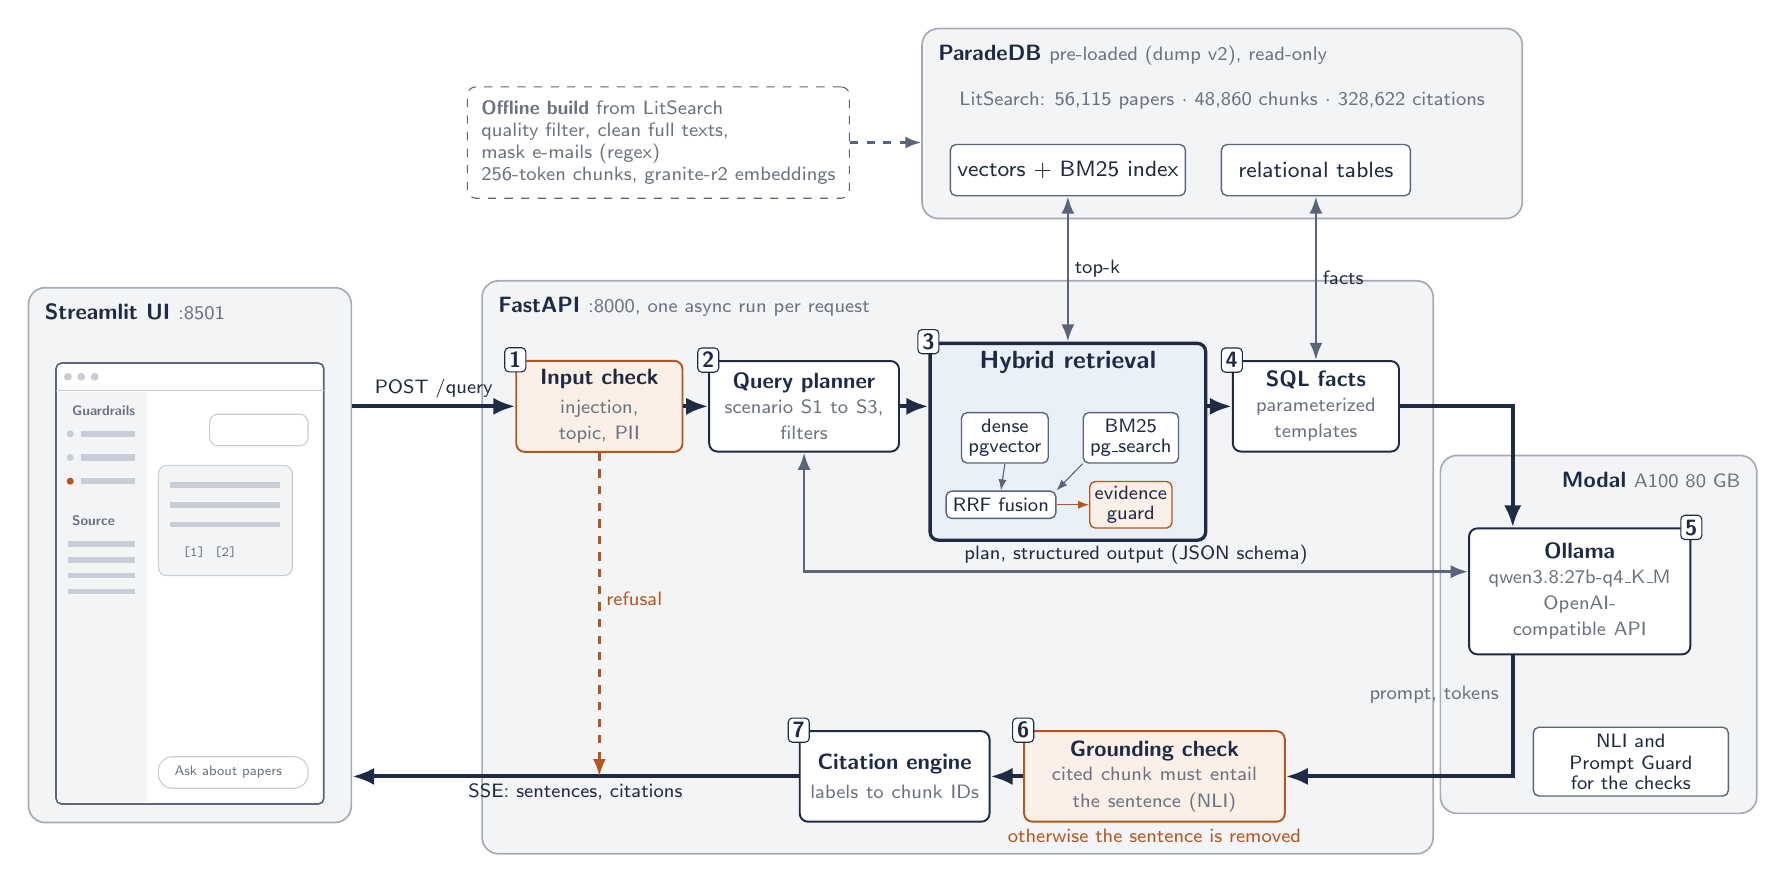
\begin{tikzpicture}

% ---------- FastAPI: the loop runs clockwise through it
\node[guard] (in)  at (6.15, -0.9) {\bx{Input check}{injection, topic, PII}};
\node[box]   (pl)  at (8.75, -0.9) {\bx{Query planner}{scenario S1 to S3,\\filters}};
\node[draw=ink, line width=1.2pt, rounded corners=3pt, fill=focus, minimum width=3.5cm,
      minimum height=2.5cm] (ret) at (12.1, -1.35) {};
\node[anchor=north, font=\small\bfseries] at (ret.north) {Hybrid retrieval};
\node[chip] (dense) at ([xshift=-0.8cm, yshift=0.05cm]ret.center) {dense\\[-1pt]pgvector};
\node[chip] (bm25)  at ([xshift=0.8cm, yshift=0.05cm]ret.center)  {BM25\\[-1pt]pg\_search};
\node[chip] (rrf)   at ([xshift=-0.85cm, yshift=-0.8cm]ret.center) {RRF fusion};
\node[chip, draw=accent, fill=accentbg, inner sep=1.8pt] (evg) at ([xshift=0.8cm, yshift=-0.8cm]ret.center) {evidence\\[-1pt]guard};
\draw[-{Latex[length=1.4mm]}, draw=line] (dense.south) -- (rrf.north);
\draw[-{Latex[length=1.4mm]}, draw=line] (bm25.south west) -- (rrf.north east);
\draw[-{Latex[length=1.4mm]}, draw=accent] (rrf.east) -- (evg.west);
\node[box, text width=1.9cm] (sql) at (15.25, -0.9) {\bx{SQL facts}{parameterized\\templates}};
\node[guard, text width=3.1cm] (chk) at (13.2, -5.6) {\bx{Grounding check}{cited chunk must entail\\the sentence (NLI)}};
\node[lbl, text=accent, anchor=north] (rm) at (chk.south) {otherwise the sentence is removed};
\node[box]   (cit) at (9.9, -5.6)  {\bx{Citation engine}{labels to chunk IDs}};
\begin{scope}[on background layer]
  \node[area, fit=(in)(sql)(chk)(cit)(ret)(rm), inner xsep=12pt, inner ysep=12pt, yshift=10pt] (api) {};
\end{scope}
\node[atitle] at (api.north west) {\textbf{FastAPI} {\scriptsize\color{muted}:8000, one async run per request}};

% ---------- Streamlit, sketched as its layout
\begin{scope}[shift={(-0.75, -0.35)}]
  \draw[draw=line, line width=0.6pt, fill=white, rounded corners=2pt] (0, 0) rectangle (3.4, -5.6);
  \draw[draw=wire] (0, -0.35) -- (3.4, -0.35);
  \foreach \x in {0.15, 0.32, 0.49} \fill[wire] (\x, -0.175) circle (0.05);
  \fill[band] (0.02, -0.37) rectangle (1.15, -5.58);
  \node[font=\tiny\bfseries, anchor=west, text=muted] at (0.08, -0.6) {Guardrails};
  \foreach \y/\c in {-0.9/wire, -1.2/wire, -1.5/accent} {
    \fill[\c] (0.18, \y) circle (0.045);
    \fill[wire] (0.32, \y-0.04) rectangle (1.0, \y+0.04);
  }
  \node[font=\tiny\bfseries, anchor=west, text=muted] at (0.08, -2.0) {Source};
  \foreach \y in {-2.3, -2.5, -2.7, -2.9} \fill[wire] (0.15, \y-0.035) rectangle (1.0, \y+0.035);
  % chat
  \draw[draw=wire, fill=white, rounded corners=3pt] (1.95, -0.65) rectangle (3.2, -1.05);
  \draw[draw=wire, fill=band, rounded corners=3pt] (1.3, -1.3) rectangle (3.0, -2.7);
  \foreach \y in {-1.55, -1.8, -2.05} \fill[wire] (1.45, \y-0.035) rectangle (2.85, \y+0.035);
  \node[font=\ttfamily\tiny, text=muted] at (1.75, -2.4) {[1]};
  \node[font=\ttfamily\tiny, text=muted] at (2.15, -2.4) {[2]};
  \draw[draw=wire, fill=white, rounded corners=5pt] (1.3, -5.0) rectangle (3.2, -5.4);
  \node[font=\tiny, text=muted, anchor=west] at (1.38, -5.2) {Ask about papers};
\end{scope}
\begin{scope}[on background layer]
  \node[area, minimum width=4.1cm, fit={(-0.75,0.15)(2.65,-6.15)}, inner sep=7pt, yshift=6pt] (ui) {};
\end{scope}
\node[atitle] at (ui.north west) {\textbf{Streamlit UI} {\scriptsize\color{muted}:8501}};

% ---------- Inference server on Modal
\node[box, text width=2.6cm, minimum height=1.6cm] (llm) at (18.6, -3.25)
  {\bx{Ollama}{qwen3.8:27b-q4\_K\_M\\OpenAI-compatible API}};
\node[chip, text width=2.3cm] (gpu) at ([xshift=0.65cm, yshift=-1.35cm]llm.south)
  {NLI and Prompt Guard\\[-1pt]for the checks};
\begin{scope}[on background layer]
  \node[area, fit=(llm)(gpu), inner xsep=10pt, inner ysep=16pt, yshift=10pt, minimum height=3.6cm] (modal) {};
\end{scope}
\node[atitle, anchor=north east] at (modal.north east) {\textbf{Modal} {\scriptsize\color{muted}A100 80 GB}};

% ---------- ParadeDB, filled before any request
\node[chip, font=\footnotesize, minimum width=2.9cm, minimum height=0.65cm] (vec) at (12.1, 2.1) {vectors + BM25 index};
\node[chip, font=\footnotesize, minimum width=2.4cm, minimum height=0.65cm] (rel) at (15.25, 2.1) {relational tables};
\node[font=\scriptsize, text=muted, anchor=west] (stats) at ([yshift=0.55cm]vec.north west) {LitSearch: 56,115 papers $\cdot$ 48,860 chunks $\cdot$ 328,622 citations};
\begin{scope}[on background layer]
  \coordinate (dbtop) at ([yshift=0.4cm]stats.north west);
  \node[area, fit=(vec)(rel)(stats)(stats.east)(dbtop), inner xsep=10pt, inner ysep=8pt] (db) {};
\end{scope}
\node[atitle] at (db.north west) {\textbf{ParadeDB} {\scriptsize\color{muted}pre-loaded (dump v2), read-only}};
\node[draw=line, dashed, rounded corners=3pt, align=left, font=\scriptsize, text=muted,
      inner sep=5pt] (build) at (6.9, 2.45)
  {\textbf{Offline build} from LitSearch\\quality filter, clean full texts,\\mask e-mails (regex)\\256-token chunks, granite-r2 embeddings};
\draw[-{Latex[length=2mm]}, draw=line, dashed, line width=0.8pt] (build) -- (build -| db.west);

% ---------- The loop
\draw[flow] (ui.east |- in.west) -- node[lbl, above] {POST /query} (in.west);
\draw[flow] (in) -- (pl);
\draw[flow] (pl.east) -- (pl.east -| ret.west);
\draw[flow] (ret.east |- sql.west) -- (sql.west);
\draw[flow] (sql.east) -| ([xshift=-0.85cm]llm.north);
\draw[flow] ([xshift=-0.85cm]llm.south) |- (chk.east);
\draw[flow] (chk) -- (cit);
\draw[flow] (cit.west) -- node[lbl, below] {SSE: sentences, citations} (cit.west -| ui.east);

% ---------- Calls to other parts
\draw[call] (pl.south) |- node[lbl, above, pos=0.75] {plan, structured output (JSON schema)} ([yshift=0.25cm]llm.west);
\draw[call] (ret.north |- vec.south) -- node[lbl, right] {top-k} ([xshift=0pt]ret.north);
\draw[call] (rel.south) -- node[lbl, right] {facts} (sql.north);
\node[lbl, anchor=east, text=muted] at ([xshift=-0.95cm, yshift=-0.5cm]llm.south) {prompt, tokens};

% Refusal leaves the loop early
\draw[-{Latex[length=2.2mm]}, draw=accent, line width=1.1pt, dashed] (in.south) --
  node[lbl, right, text=accent, pos=0.45] {refusal} (in.south |- cit.west);

% Order
\tagged{in}{1}
\tagged{pl}{2}
\tagged{ret}{3}
\tagged{sql}{4}
\node[tag] at (llm.north east) {5};
\tagged{chk}{6}
\tagged{cit}{7}

\end{tikzpicture}
\end{document}
